\section{Contexte et études préliminaires}
\ifprof
\else
Les progrès en mécatronique et les systèmes numériques (vision, commande, etc.) associés à la robotique ont permis le développement de systèmes robotisés qui apportent une aide au geste chirurgical et permettent la diminution des traumatismes opératoires. Ce développement de robots dédiés aux applications chirurgicales est en progression depuis les années 1980 même si les aspects purement économiques sont difficiles à évaluer en raison de la multitude de critères à prendre en compte: cout du robot et de sa maintenance, réduction de la durée d'hospitalisation, suivi post-opératoire, diminution de la taille des cicatrices, etc.\\
Ainsi, le développement de ces systèmes ne se réduit pas aux seuls aspects économiques, d'autres critères (diminution du traumatisme opératoire, du temps de récupération, du saignement, etc.) entrent en jeu. Du point de vue de la robotique, de nombreux travaux de recherche actuels portent sur l'amélioration de la précision du geste chirurgical en prenant en compte dans la commande du robot les mouvements physiologiques (périodiques) du patient comme les mouvements respiratoires ou ceux dus aux battements cardiaques. Ces mouvements perturbent le geste chirurgical, en particulier lorsqu'un niveau de précision important est exigé.\\
Pour répondre à ce problème, différentes solutions peuvent être envisagées. L'une d'elles consiste à faire suivre à l'instrument un mouvement périodique synchronisé avec les mouvements physiologiques de la zone d'opération considérée. Un système de mesure et de traitement de l'information (hors du cadre de cette étude) permet de restituer au chirurgien une image virtuelle assimilable à une opération sur un organe fixe. Une des difficultés (objet des travaux de recherche actuels) réside dans le développement de systèmes robotisés et de méthodes de commande fiables aptes à assurer le déplacement synchrone du robot avec les mouvements physiologiques et avec le niveau de précision requis.

Dans ce contexte, le Service d'Automatique et d'Analyse des Systèmes (SAAS) de l'École polytechnique de Bruxelles (au sein de l'Université Libre de Bruxelles) mène des travaux de recherche sur le développement de robots de chirurgie mini-invasive. L'objectif de ces travaux s'inscrit dans le développement d'une architecture de commande d'un système télé-opéré afin que le robot compense les mouvements physiologiques dus à la respiration (objet de cette étude) et transmette au chirurgien un effort représentatif du contact entre les outils chirurgicaux et leur environnement, de façon à reproduire un ressenti semblable à celui d'une chirurgie traditionnelle afin d'éviter de blesser les organes du patient.

\begin{figure}[!h]
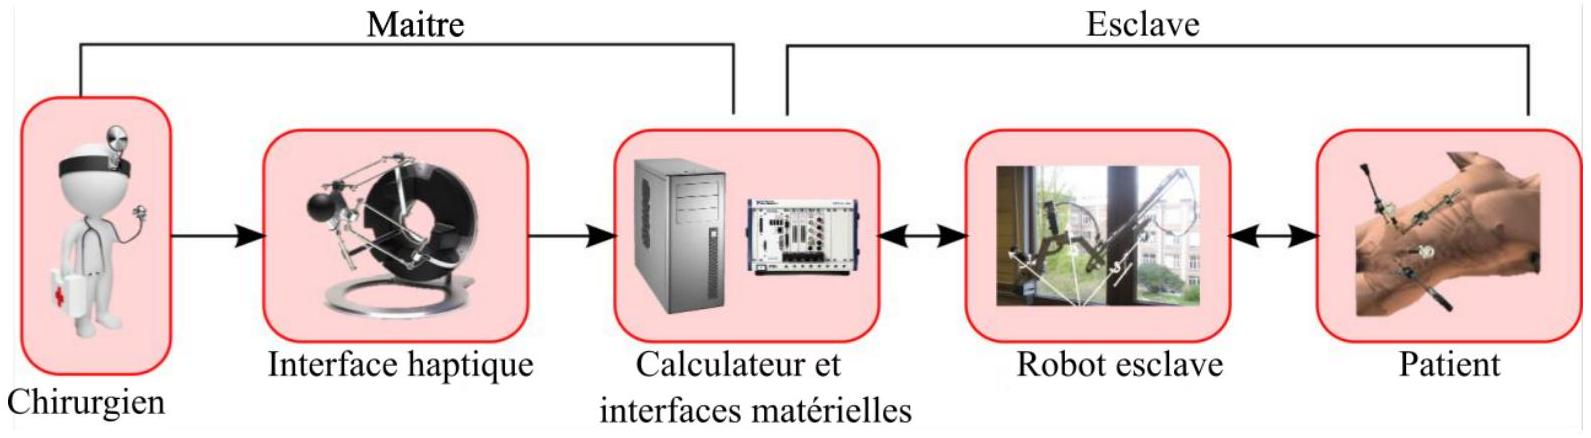
\includegraphics[width=\textwidth]{2025_07_10_a3cef788f652ce14ded2g-01}
\centering
%Figure 1 
\caption{Structure d'un robot pour la chirurgie mini-invasive\label{ccs_psi_2019_fig_01}}
\end{figure}

La structure fonctionnelle du système robotisé développée par l'équipe du SAAS pour la chirurgie robotisée est représentée sur la figure \ref{ccs_psi_2019_fig_01}. Elle est composée en particulier :

\begin{itemize}
  \item d'une interface haptique (robot maitre) permettant de générer les consignes d'un robot esclave à partir des mouvements du chirurgien et effectuant un retour d'effort permettant de restituer l'effort de contact entre les instruments chirurgicaux et l'environnement ;
  \item d'un robot esclave reproduisant les mouvements pilotés par le chirurgien.
\end{itemize}


En pratique, les consignes de déplacement du robot sont générées :
\begin{itemize}
  \item à partir d'une estimation des mouvements physiologiques de l'organe considéré à suivre ;
  \item auxquels sont ajoutés les déplacements demandés par le chirurgien.
\end{itemize}

Le cadre de ce sujet porte plus spécifiquement sur l'analyse de la pertinence de l'architecture robotisée à satisfaire l'objectif de la compensation des mouvements physiologiques dus à la respiration. Il s'agit donc d'étudier et d'analyser la structure de commande du robot permettant de suivre les déplacements physiologiques et ceux commandés par le chirurgien. Le sujet est décomposé en 4 parties ;

\begin{itemize}
  \item dans la partie I, une analyse des signaux physiologiques sera effectuée et le cahier des charges de la chaine d'asservissement sera complété par la description des propriétés des signaux physiologiques ;
  \item le développement d'un modèle dynamique dans l'objectif de la définition et de la synthèse d'une loi de commande permettant d'asservir le robot esclave sera l'objet de la partie II ;
  \item la partie III portera sur la conception d'une loi de commande de base, en exploitant le modèle dynamique développé dans la partie II. Le but sera d'asservir le déplacement du robot aux consignes obtenues par l'addition des mouvements physiologiques périodiques et du déplacement demandé par le chirurgien dans le repère fixe virtuel ;
  \item enfin, dans la partie IV, une adaptation de la loi de commande de base sera envisagée en vue d'assurer le suivi des mouvements physiologiques avec le niveau de précision requis par le cahier des charges.
\end{itemize}
\fi

%I 
\section{Analyse des propriétés des signaux physiologiques}
%\section*{Objectif}

\begin{obj}
Analyser les propriétés des signaux physiologiques et en déduire des éléments du cahier des charges de la loi de commande pour assurer le déplacement du robot avec le niveau de précision requis.
\end{obj}

\ifprof
\else
L'architecture de commande adoptée dans le cadre de ce projet est illustrée par le schéma de la figure \ref{ccs_psi_2019_fig_02} :

\begin{itemize}
  \item le robot esclave est piloté en position dans le repère articulaire (et non directement dans le repère cartésien), au moyen de l'asservissement des positions angulaires $\mathbf{q}$ des différentes articulations, car les mesures utilisées sont les angles des arbres moteurs ;
  \item les composantes cartésiennes de la consigne de déplacement $\mathbf{X}^{*}=\mathbf{X}_{\mathbf{c h}}^{*}+\boldsymbol{\delta} \mathbf{X}_{\text {org }}$ sont générées par le chirurgien au moyen du robot maitre (composante $\mathbf{X}_{\mathrm{ch}}^{*}$ ) et auxquelles on rajoute les déplacements (composante $\boldsymbol{\delta} \mathbf{X}_{\text {org }}$ ) pour le suivi synchrone des mouvements physiologiques de l'organe considéré ;
  \item cette prise en compte des mouvements physiologiques est utilisée de façon à ce que l'asservissement en position du robot esclave permette de suivre ces mouvements se traduisant ainsi par leur compensation au regard du geste du chirurgien ;
  \item la mesure $\mathbf{F}_{\mathrm{s}}$ au moyen d'un capteur d'effort permet de réaliser une restitution d'effort au chirurgien.
\end{itemize}


\begin{figure}[!h]
\centering
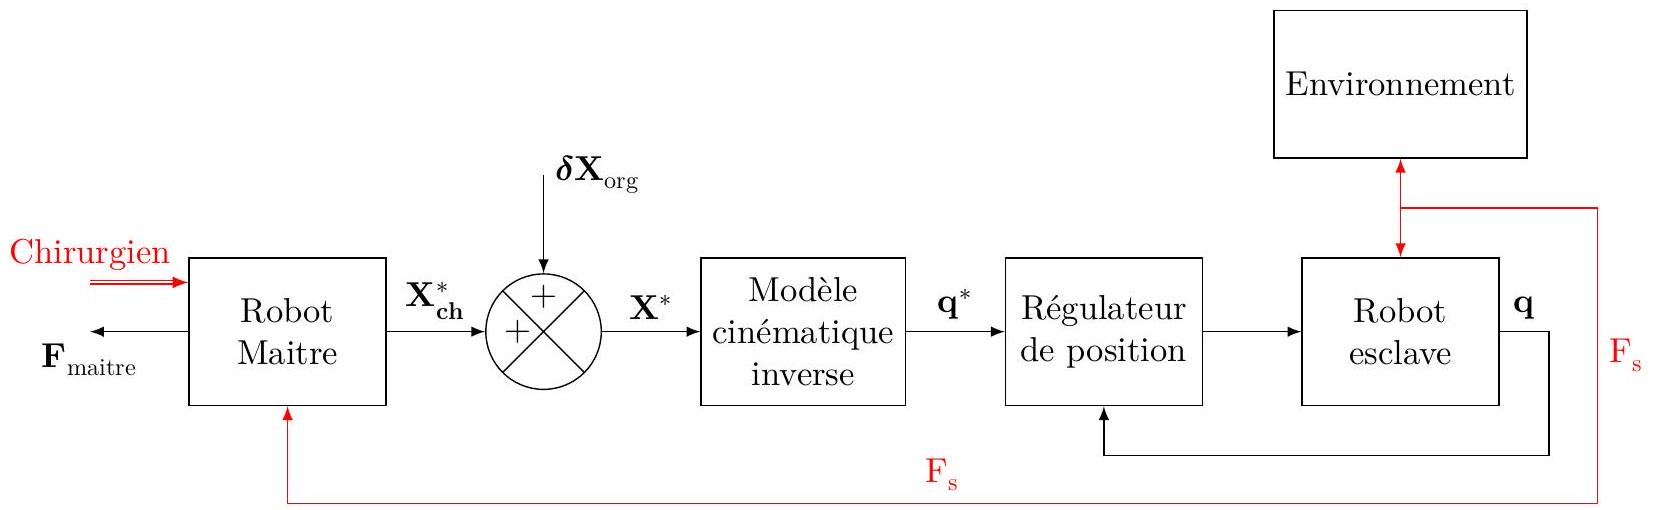
\includegraphics[width=\textwidth]{2025_07_10_a3cef788f652ce14ded2g-02}

%Figure 2 \\
\caption{Principe de la commande du robot de téléopération\label{ccs_psi_2019_fig_02}}
\end{figure}



L'objet de cette partie est d'analyser les propriétés des signaux physiologiques et de compléter partiellement le cahier des charges de la chaine d'asservissement en position du robot esclave. Le contexte abordé concerne plus particulièrement celui des cas d'opérations avec assistance respiratoire.\\
Les exigences du cahier des charges sont indiquées sur le diagramme de la figure \label{ccs_psi_2019_fig_03}. Les exigences 1.3.1 et 1.3.2 seront à préciser dans les questions 1 à 6 .


\begin{figure}[!h]
\centering
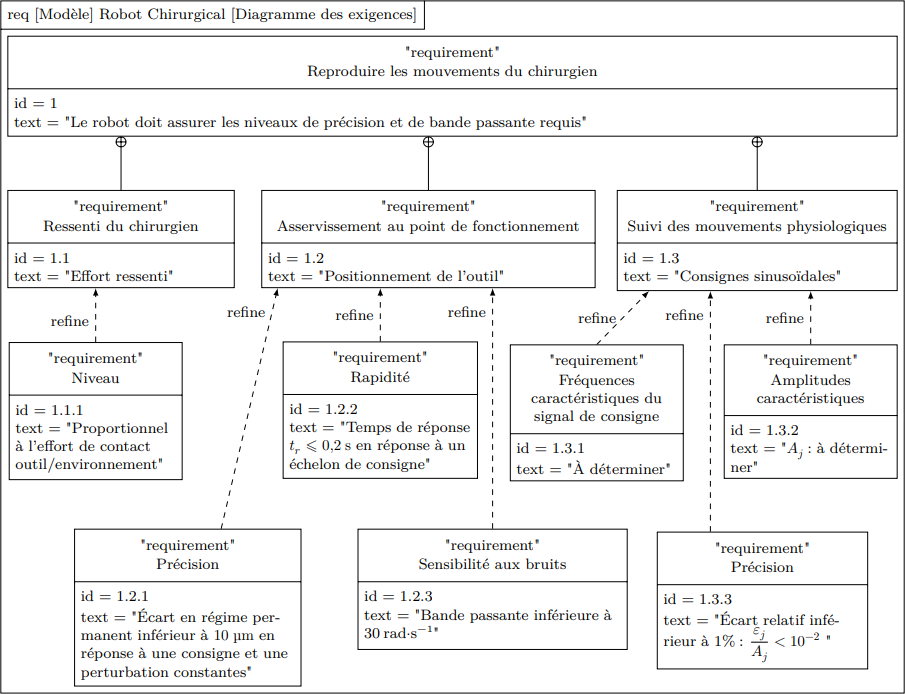
\includegraphics[width=\textwidth]{req}

%Figure 3 \\
\caption{Cahier des charges\label{ccs_psi_2019_fig_03}}
\end{figure}
\fi


%I.A - 
\subsection{Analyse des propriétés des signaux des mouvements physiologiques}
%\section*{Objectif}
\begin{obj}
Proposer un algorithme permettant de mettre en évidence les propriétés des mouvements respiratoires.
\end{obj}

\ifprof
\else
Un enregistrement expérimental des mouvements physiologiques dus à la respiration est donné sur la figure \ref{ccs_psi_2019_fig_04} montrant les déplacements de l'organe considéré dans cette étude.


\begin{figure}[!h]
\centering
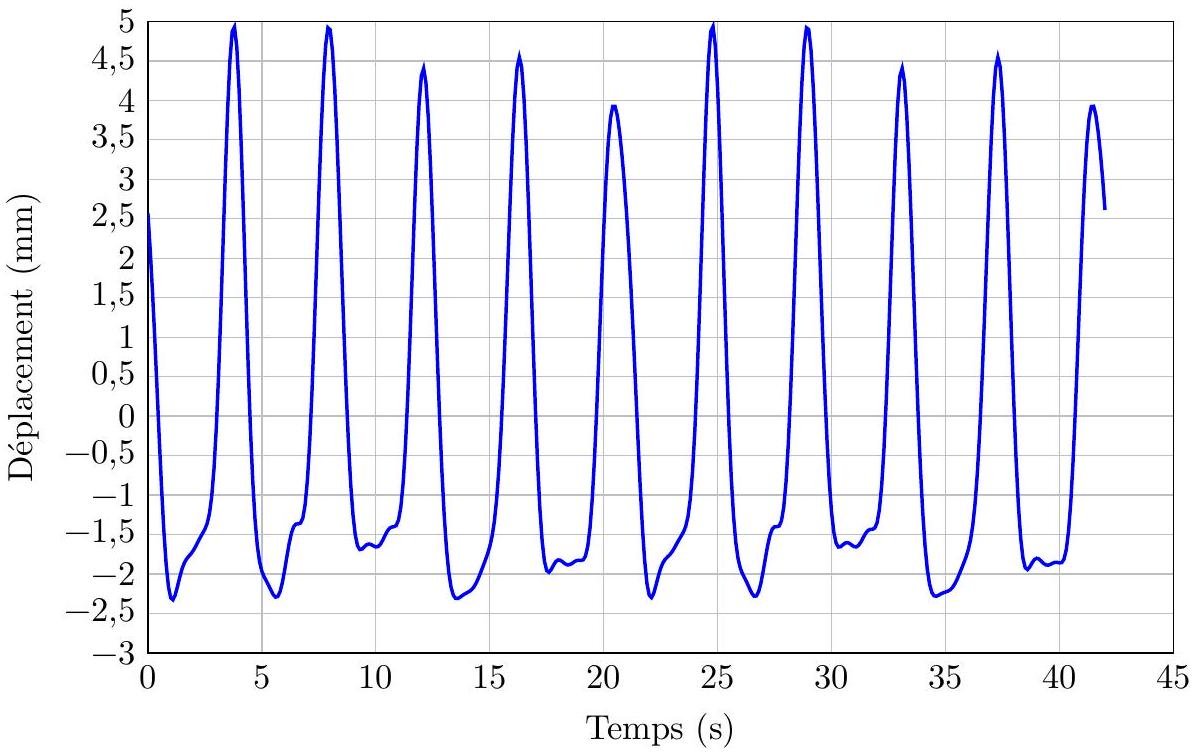
\includegraphics[width=\textwidth]{2025_07_10_a3cef788f652ce14ded2g-03(1)}

%Figure 4 \\
\caption{Déplacement dû aux mouvements physiologiques\label{ccs_psi_2019_fig_04}}
\end{figure}
\fi

%Q 1. 
\question{Commenter l'allure de ce signal en précisant ses principales caractéristiques à considérer pour le calcul d'une loi de commande performante de la chaine d'asservissement.}
\ifprof
\begin{corrige}
Le signal semble presque periodique même si les amplitudes des déplacements ne sont pas exactement les mêmes.
L'amplitude maximale obtenue est d'environ $\dfrac{5+2,3}{2}=\SI{3,65}{mm}$ et l'amplitude minimale obtenue est d'environ : $\dfrac{4+2}{2}=\SI{3}{mm}$. 
La période des oscillation est d'environ $
T\approx\dfrac{41-4}{9}\approx \SI{4,1}{s}$. 
Soit une pulsation de $\omega\approx \SI{1,53}{rad.s^{-1}}$.
\end{corrige}
\else
\fi

\ifprof
\else
Afin d'analyser les propriétés des mouvements respiratoires, une solution possible est d'analyser le contenu spectral du signal considéré. Pour cela, on peut utiliser la transformation de Fourier qui peut être appliquée à un signal quelconque, non nécessairement périodique, sur une fenêtre de temps finie. Si on note un signal temporel $s(t)$, sa transformée de Fourier $S(f)$ est donnée par $S(f)=\int_{-\infty}^{\infty} s(t) \mathrm{e}^{-\mathrm{i} 2 \pi f t} \mathrm{~d} t$ où $S(f)$ est une fonction complexe de la fréquence $f$. D'un point de vue du traitement numérique, le contenu spectral est estimé en utilisant un enregistrement sur une durée limitée $t \in\left[0, t_{\max }\right]$. La relation normée suivante permet d'obtenir directement les amplitudes des différentes composantes harmoniques

$$
\hat{S}(f)=\frac{1}{N} \sum_{k=0}^{N-1} s\left[k T_{e}\right] \mathrm{e}^{-\mathrm{i} 2 \pi f T_{e} k}
$$

où $T_{e}$ est la période d'échantillonnage, $s\left[k T_{e}\right]$ représente l'échantillon de $s(t)$ à l'instant $t=k T_{e}, f$ est la fréquence considérée, $N$ et $t_{\max }$ sont choisis tels que $t_{\max }=(N-1) T_{e}$. Le calcul du spectre est réalisé pour un ensemble de fréquences tel que :

$$
E_{f}={ }^{t}\left(\begin{array}{lllll}
0 & f_{1} & f_{2} & \cdots & f_{N_{f}-1}
\end{array}\right)
$$

où $f_{N_{f}-1}=f_{\max } \leqslant \frac{1}{2 T_{e}}$. L'ensemble de fréquences peut, par exemple, être choisi selon une distribution linéaire, $\left\{f_{n}=n \delta f ; n=0, \cdots, N_{f}-1\right\}$ avec $\delta f$ choisi tel que $f_{\max }=\left(N_{f}-1\right) \delta f, N_{f}$ est le nombre d'éléments de $E_{f}$.\\
Dans ce contexte, $\hat{S}\left(f_{n}\right)$ est un nombre complexe

\begin{itemize}
  \item dont le module est une estimation de l'amplitude de la composante sinusoïdale $s_{n}(t)=A_{n} \sin \left(2 \pi f_{n} t+\Phi_{n}\right)$, soit $A_{n}=2\left\|\hat{S}\left(f_{n}\right)\right\|$, à la fréquence $f_{n}$ du signal $s(t)$;
  \item et l'argument est la phase $\Phi_{n}$.
\end{itemize}

Le signal $s(t)$ peut être alors approché sous la forme $\sum_{n=0}^{N_{f}-1} s_{n}(t)$.\\
On note $S_{p}={ }^{t}\left(\begin{array}{lllll}\hat{S}(0) & \hat{S}\left(f_{1}\right) & \hat{S}\left(f_{2}\right) & \cdots & \hat{S}\left(f_{N-1}\right)\end{array}\right)$ la matrice colonne contenant les composantes spectrales correspondantes aux fréquences $f_{n} \in E_{f}$ et $V_{s}=^{t}\left(s[0] \quad s\left[T_{e}\right] \quad s\left[2 T_{e}\right] \quad \cdots \quad s\left[(N-1) T_{e}\right]\right)$ une matrice colonne contenant les échantillons du signal dans la fenêtre temporelle $\left[0,(N-1) T_{e}\right]$.\\
\fi

%Q 2. 
\question{Formuler $\hat{S}\left(f_{n}\right)$ sous la forme $\hat{S}\left(f_{n}\right)=L_{n} \cdot V_{s}$ où $L_{n}$ est une matrice ligne. Exprimer les composantes $l_{k}\left(f_{n}\right)$ de la matrice $L_{n}$ en fonction de $k, T_{e}$ et des $f_{n}\left(0 \leqslant n \leqslant N_{f}-1\right)$.}
\ifprof
\begin{corrige}
D'après la définition, 
$\hat{S}\left( f_n\right)= \dfrac{1}{N_f} \sum \limits_{k=0}^{N_f-1} s\left[kT_e\right] \text{e}^{-i 2 \pi f_nT_e k}$

$= \dfrac{1}{N_f} \left(
 s\left[0 T_e\right] \text{e}^{-i 2 \pi f_nT_e 0} + 
 s\left[T_e\right] \text{e}^{-i 2 \pi f_nT_e } + ... 
 s\left[\left( N_f-1\right)T_e\right] \text{e}^{-i 2 \pi f_nT_e \left( N_f-1\right)}\right)$

$= \dfrac{1}{N_f} \left(
 s\left[0\right] + 
 s\left[T_e\right] \text{e}^{-i 2 \pi f_nT_e } + ... 
 s\left[\left( N_f-1\right)T_e\right] \text{e}^{-i 2 \pi f_nT_e \left( N_f-1\right)}\right)$.
 
 On a donc $l_k\left(f_n\right)=\dfrac{1}{N_f}\text{e}^{-i 2 \pi f_nT_e k}$.
\end{corrige}
\else
\fi

%Q 3. 
\question{Formuler $S_{p}$ sous la forme $S_{p}=M \cdot V_{s}$ où $M$ est une matrice de dimensions $N_{f} \times N$.}
\ifprof
\begin{corrige}
On a $L_n = \begin{pmatrix}  l_0 f_n  & l_1 f_n & l_2 f_n & \ldots & l_{N-1} f_n\end{pmatrix}$.
Par ailleurs, 
$S_p = 
\begin{pmatrix} \hat{S}\left( 0\right) \\ \hat{S}\left( f_1\right) \\ \hat{S}\left( f_2\right)  \\ \vdots \\ \hat{S}\left( f_{N-1}\right) \end{pmatrix} 
=
\begin{pmatrix} 
L_0 V_s \\
L_1 V_s \\
L_2 V_s \\
\vdots \\
 L_{N-1} V_s\end{pmatrix}$.

On a donc $ L_{k} V_s =\begin{pmatrix}  l_0 f_k  & l_1 f_k & l_2 f_k & \ldots & l_{N-1} f_k\end{pmatrix} \begin{pmatrix}
s[0]  \\ s[T_e] \\ s[2T_e] \\ \vdots \\ s\left[\left(N-1\right)T_e\right] \\   \end{pmatrix} = \sum  \limits_{i=0}^{N-1} l_i f_k s\left[i T_e\right]$.


Ainsi la matrice $M$ est composé de toutes les lignes $L_n$ pour $n\in  \llbracket 0,N_f-1\rrbracket$.
La matrice $M$ aura donc pour forme : 

$
M=\dfrac{1}{N_f}
\left(
\begin{array}{cccc}
1 & 1 & \ldots & 1 \\ 
1 & e^{-i2\pi f_1T_e} & \ldots & e^{-i2\pi f_{1}T_e(N-1)} \\ 
\vdots & e^{-i2\pi f_nT_e} & \ldots & e^{-i2\pi f_{n}T_e(N-1)} \\ 
1 & e^{-i2\pi f_{N_f-1}T_e} & \ldots & e^{-i2\pi f_{N_f-1}T_e(N-1)} \\ 
\end{array} 
\right)
$.
\end{corrige}
\else
\fi

%Q 4. 
\question{Exprimer les coefficients $a_{n, m}$ de $M$ en fonction de $m, T_{e}$ et des $f_{n}\left(0 \leqslant n \leqslant N_{f}-1\right)$.}
\ifprof
\begin{corrige}
De la question précédente, on peut exprimer le terme $a_{n,m}$  : 

$a_{n,m}=\dfrac{1}{N_f}e^{-i2\pi f_{n}T_em}$.
\end{corrige}
\else
\fi

%Q 5. 
\question{Exprimer la matrice $M$ en fonction de $E_{f}$ et de la matrice ligne $t_{k}=\left(\begin{array}{lllll}0 & T_{e} & 2 T_{e} & \cdots & (N-1) T_{e}\end{array}\right)$ contenant les instants d'échantillonnage $k T_{e}$ dans la fenêtre temporelle $\left[0,(N-1) T_{e}\right]$.
On pourra noter $\exp (\mathbf{X})$ la matrice obtenue en prenant l'exponentielle $\mathrm{e}^{x_{i, j}}$ de chacun des coefficients de
la matrice $\mathbf{X}$. la matrice $\mathbf{X}$.}
\ifprof
\begin{corrige}
En posant 
$
X=-i2\pi
\left(
\begin{array}{c}
0\\
f_1\\
f_2\\
\vdots\\
f_{N_f-1}
\end{array}
\right)
\cdot
\left(
\begin{array}{ccccc}
0& T_e & 2T_e &\ldots & (N-1)T_e
\end{array}
\right)
=-i2\pi E_f\cdot t_k
$, on obtient bien, $
M=\dfrac{1}{N_f}\exp(X)$.
\end{corrige}
\else
\fi

%Q 6. 
\question{En utilisant le langage Python, écrire une fonction calculSpectre d'entête 
\lstinline{def calculSpectre(Signal:np.ndarray, Nf:int, fmax:float, Te:float) -> np.ndarray:}
qui renvoie un vecteur contenant les amplitudes $A_{n}$ des $N_{f}$ composantes sinusoïdales distribuées linéairement entre 0 et fmax. Cette fonction prend en paramètres le vecteur Signal contenant les $N$ échantillons du signal pris dans la fenêtre temporelle objet de la mesure, le nombre Nf de points pour le calcul du spectre, la fréquence maximale fmax considérée pour le calcul et la période d'échantillonnage Te.}
\ifprof
\begin{corrige}
\begin{lstlisting}
import numpy as np
def calculSpectre(Signal,Nf,fmax,Te):
    Vs=np.transpose([np.array(Signal)])
    Ef=np.transpose([np.linspace(0,fmax,Nf)])
    tk=np.array([range(len(Signal))])*Te
    X=np.dot(Ef,tk)*(-1j*2*np.pi)
    M=1/Nf*np.exp(X)
    Sp=np.dot(M,Vs)
    An=abs(Sp)
    return An
\end{lstlisting}
\end{corrige}
\else
\fi

\ifprof
\else

Une liste (non exhaustive) de fonctions Python permettant de manipuler des tableaux et des nombres complexes est donnée dans le document réponse.\\
L'application de cette procédure au signal enregistré conduit au contenu spectral représenté sur la figure \ref{ccs_psi_2019_fig_05} . L'analyse de ce contenu fait apparaitre deux composantes principales aux fréquences $f_{1}=0,24 \mathrm{~Hz}$ et $f_{2}=0,48 \mathrm{~Hz}$ d'amplitudes respectives $A_{1}=2,94 \mathrm{~mm}$ et $A_{2}=1,30 \mathrm{~mm}$. Dans la suite de cette partie, on ne prend en compte qu'une seule composante et on modélise le mouvement respiratoire sous la forme d'un signal de déplacement $z^{*}(t)=A_{2} \sin \left(2 \pi f_{2} t+\Phi_{2}\right)$, correspondant au cas le plus contraignant en terme de performance.


\begin{figure}[!h]
\centering
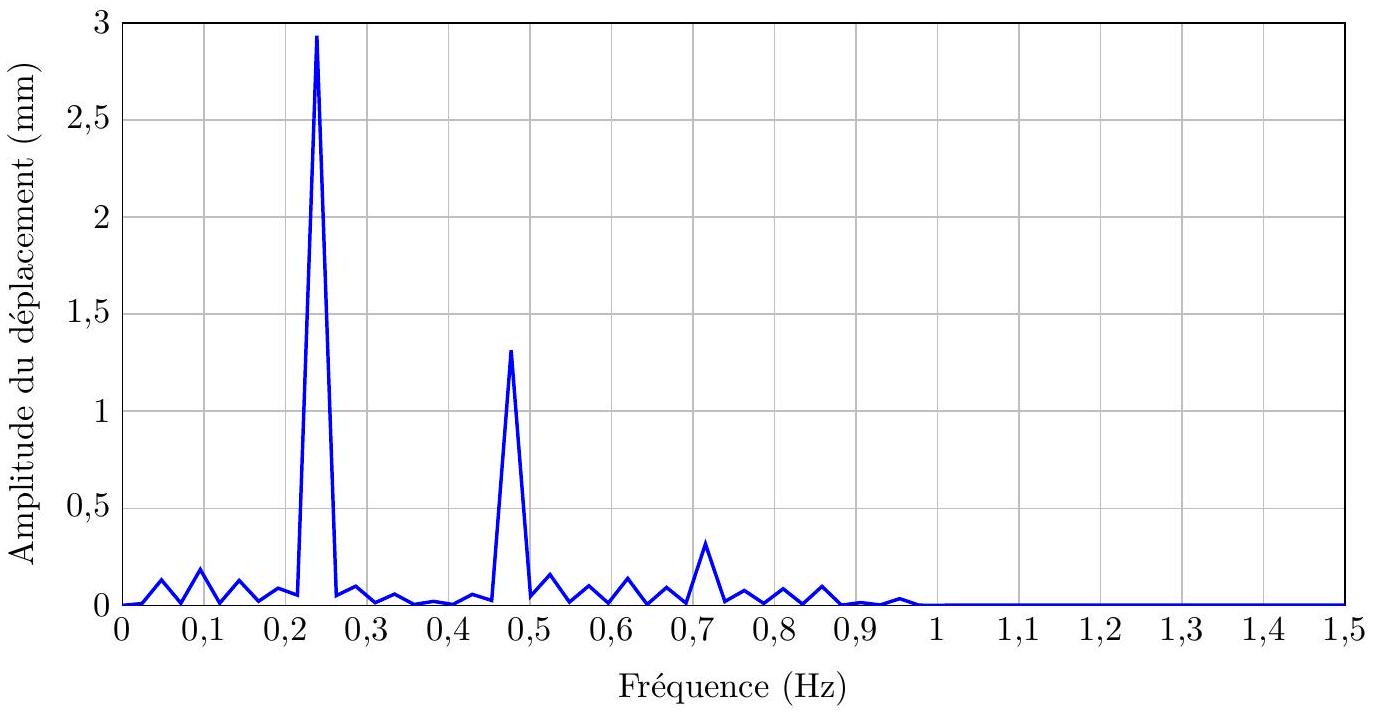
\includegraphics[width=\textwidth,]{2025_07_10_a3cef788f652ce14ded2g-05}

%Figure 5 \\
\caption{Contenu spectral du déplacement dû aux mouvements physiologiques\label{ccs_psi_2019_fig_05}}
\end{figure}


\fi

